\documentclass[de]{./../../common/SurferDesc}%%%%%%%%%%%%%%%%%%%%%%%%%%%%%%%%%%%%%%%%%%%%%%%%%%%%%%%%%%%%%%%%%%%%%%%
%
% The document starts here:
%
\begin{document}
\footnotesize
% Weltrekordfl�chen

%%% 1.Tafel

%%%%%%%%%%%%%%%%%%%%%%%%%%%%%


\begin{surferPage}
  \begin{surferTitle}Fl�chen mit vielen reellen Singularit�ten\end{surferTitle}   \\
  Wie bereits erw�hnt, ist schon f�r Fl�chen von Grad $7$ unbekannt, was die
    maximale Anzahl $\mu(7)$ von singul�ren Punkten darauf ist; man wei� derzeit
    nur, dass $99\le \mu(7) \le 104$ gilt. 

    Daher erstaunt es nicht, dass man f�r beliebigen Grad $d$ noch weniger
    wei�.
    Sonja Breske, Oliver Labs und Duco van Straten konnten 2005 wenigstens eine
    Konstruktion von S.V.\ Chmutov so ver�ndern, dass das bisher bekannte
    Maximum von Singularit�ten, $\mu(d)$, nun auch mit reellen Singularit�ten 
    erreicht wird.
    Man wei� daher bisher: 
    \[0,41\bar{6}d^3 \lessapprox \mu(d) \lessapprox 0.44\bar{4} d^3.\]
    Von oben erkennt man sch�n die Symmetrie der Konstruktion
    und ihren Zusammenhang mit der Frage nach der maximalen Anzahl schwarzer
    Zellen in einem Arrangement von Geraden:
    \begin{center}
      \begin{tabular}{c@{\qquad}c}
        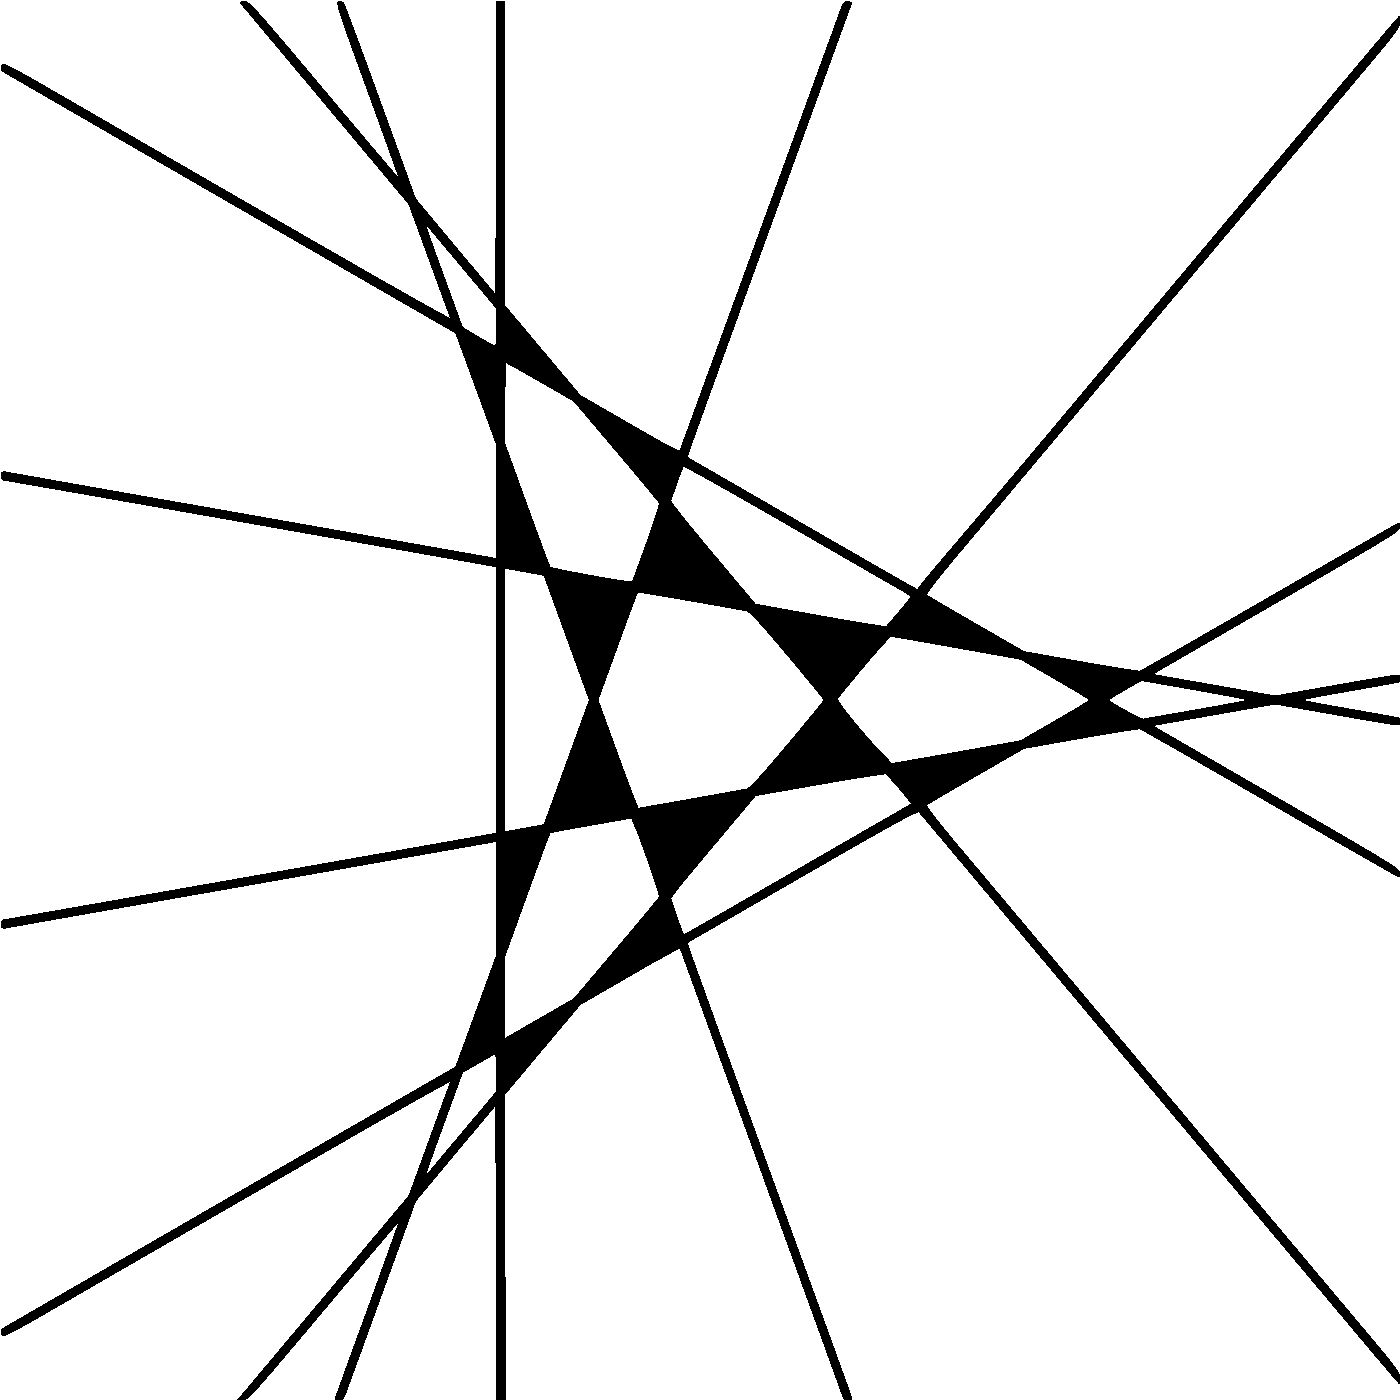
\includegraphics[height=1.5cm]{./../../common/images/vielesing.pdf}
        &
        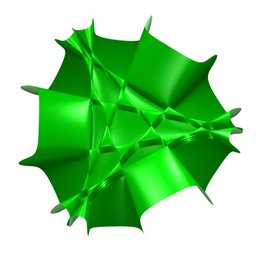
\includegraphics[height=1.5cm]{./../../common/images/p9surface_von_oben}
      \end{tabular}
    \end{center}

  \begin{surferText}
     \end{surferText}
\end{surferPage}
%%%%%%%%%%%%%%%%%%%%%%%%%%%%%

\end{document}
%
% end of the document.
%
%%%%%%%%%%%%%%%%%%%%%%%%%%%%%%%%%%%%%%%%%%%%%%%%%%%%%%%%%%%%%%%%%%%%%%%
